\documentclass[
  unicode,a4paper,9pt,
  % aspectratio=169,
  xcolor = {dvipsnames,svgnames},
  hyperref ={colorlinks=true,citecolor=Navy,linkcolor=NavyBlue,urlcolor=purple},
  ja=standard,lualatex
]{beamer}
\renewcommand{\baselinestretch}{1.4}

% ---fonts---
\PassOptionsToPackage{quiet}{fontspec}
\usefonttheme{serif}
\mathversion{bold}
\usepackage{luatexja-fontspec}
\setmainfont{TeX Gyre Termes}
\setmainjfont{Noto Sans CJK JP}
% \setmainjfont[BoldFont = HaranoAjiGothic-Regular]{HaranoAjiMincho}
% \setmainjfont[BoldFont = IPAGothic]{IPAMincho}
\setmathrm{Latin Modern Roman}
% \usepackage{newtxmath}

\usepackage{newunicodechar}
\newunicodechar{–}{-}

% ---refer `texdoc xcolor' at the command line---

% ---Display \subsubsection at the Index
% \setcounter{tocdepth}{3}

% ---Setting about the geometry of the document----
% \usepackage{a4wide}
% \pagestyle{empty}

% ---Physics and Math Packages---
\usepackage{amssymb,amsfonts,amsthm,mathtools}
\usepackage{physics,braket,bm,slashed}

% ---underline---
\usepackage[normalem]{ulem}

% ---cancel---
\usepackage{cancel}

% --- surround the texts or equations
\usepackage{fancybox,ascmac}

% ---settings of theorem environment---
\usepackage{amsthm}
\theoremstyle{definition}

% ---settings of proof environment---
\renewcommand{\proofname}{\textbf{証明}}
\renewcommand{\qedsymbol}{$\blacksquare$}

% ---Insert the figure (If insert the `draft' at the option, the process becomes faster.)---
\usepackage{graphicx}
% \usepackage{subcaption}

% ----Add a link to a text---
\usepackage{url,hyperref}
\usepackage{xcolor}

% ---Tikz---
\usepackage{tikz,pgf,pgfplots,circuitikz}
\pgfplotsset{compat=1.15}
\usetikzlibrary{intersections,arrows.meta,angles,calc,3d,decorations.pathmorphing,positioning}

% ---Add the section number to the equation, figure, and table number---
\makeatletter
   \renewcommand{\theequation}{\thesection.\arabic{equation}}
   \@addtoreset{equation}{section}
   
   \renewcommand{\thefigure}{\thesection.\arabic{figure}}
   \@addtoreset{figure}{section}
   
   \renewcommand{\thetable}{\thesection.\arabic{table}}
   \@addtoreset{table}{section}
\makeatother

% ---enumerate---
% \renewcommand{\labelenumi}{$\arabic{enumi}.$}
% \renewcommand{\labelenumii}{$(\arabic{enumii})$}

% ---beamer settings---
\usefonttheme{professionalfonts}
\usecolortheme{seahorse}
\setbeamercolor{structure}{fg=white}
\setbeamercolor{local structure}{fg=red}
\setbeamertemplate{itemize item}[ball]
\setbeamertemplate{enumerate item}[circle]
\setbeamercolor{bibliography entry author}{fg=black}
\setbeamercolor{bibliography item}{fg=black}
\setbeamercolor{alerted text}{fg=RoyalBlue}
\setbeamertemplate{frametitle continuation}{}
\setbeamertemplate{footline}[frame number]
\setbeamertemplate{navigation symbols}{} 
\setbeamersize{text margin left=10pt, text margin right=10pt}

% ---tcolorbox---
\usepackage{tcolorbox}
\tcbuselibrary{theorems}
\tcbuselibrary{raster}
\tcbuselibrary{skins}
\newtcolorbox{bluebox}[2][]{enhanced,
colframe=RoyalBlue!40!white,
colback=RoyalBlue!10!white,
coltitle=black,
drop fuzzy shadow, title={#2}
,#1}
\newtcolorbox{redbox}[2][]{enhanced,
colframe=DarkRed!40!white,
colback=DarkRed!10!white,
coltitle=black,
drop fuzzy shadow, title={#2}
,#1}

% ---tcolorbox---
\usepackage{tcolorbox}
\tcbuselibrary{raster,skins,breakable}
\newtcolorbox{graybox}[1][]{frame empty, colback=black!10!white, sharp corners}

% ---Ignore the Warnings---
\usepackage{silence}
\WarningFilter{latexfont}{Some font shapes}
\WarningFilter{latexfont}{Font shape}
\WarningFilter{latexfont}{Size substitutions}
\ExplSyntaxOn
\msg_redirect_name:nnn{hooks}{generic-deprecated}{none}
\ExplSyntaxOff

% ---Citation on the slides---
\newcommand*{\citefone}[2]{
  \begin{tikzpicture}[remember picture, overlay]
    \node[anchor=north east, align=left] at ($(current page.north east)-(0,0.0)$){
    {\tiny
      \cite{#1}
      #2
    }
    };
  \end{tikzpicture}

  \vspace*{-20pt}
}

\newcommand*{\citeftwo}[4]{
  \begin{tikzpicture}[remember picture, overlay]
    \node[anchor=north east, align=left] at ($(current page.north east)-(0,0.0)$){
    {\tiny
      \cite{#1}
      #2
    }
    \\[-2.4ex]
    {\tiny
      \cite{#3}
      #4
    }
    };
  \end{tikzpicture}

  \vspace*{-20pt}
}

\newcommand*{\citefthree}[6]{
  \begin{tikzpicture}[remember picture, overlay]
    \node[anchor=north east, align=left] at ($(current page.north east)-(0,0.0)$){
    {\tiny
      \cite{#1}
      #2
    }
    \\[-2.4ex]
    {\tiny
      \cite{#3}
      #4
    }
    \\[-2.4ex]
    {\tiny
      \cite{#5}
      #6
    }
    };
  \end{tikzpicture}

  \vspace*{-20pt}
}

\newcommand*{\citefonev}[3]{
  \begin{tikzpicture}[remember picture, overlay]
    \node[anchor=north east, align=left, text width=#3cm] at ($(current page.north east)-(0,0.0)$){
    {{\fontsize{5pt}{0pt}\selectfont
      \cite{#1}
      #2\par}
    }
    };
  \end{tikzpicture}

  \vspace*{-20pt}
}

\newcommand*{\citeftwov}[5]{
  \begin{tikzpicture}[remember picture, overlay]
    \node[anchor=north east, align=left, text width=#5cm] at ($(current page.north east)-(0,0.0)$){
    {{\fontsize{5pt}{0pt}\selectfont
      \cite{#1}
      #2\par}

      {\fontsize{5pt}{0pt}\selectfont
      \cite{#3}
      #4\par}
    }
    };
  \end{tikzpicture}

  \vspace*{-20pt}
}

\newcommand*{\citefthreev}[7]{
  \begin{tikzpicture}[remember picture, overlay]
    \node[anchor=north east, align=left, text width=#7cm] at ($(current page.north east)-(0,0.0)$){
    {{\fontsize{5pt}{0pt}\selectfont
    \cite{#1}
    #2\par}

    {\fontsize{5pt}{0pt}\selectfont
    \cite{#3}
    #4\par}

    {\fontsize{5pt}{0pt}\selectfont
    \cite{#5}
    #6\par}
    }
    };
  \end{tikzpicture}

  \vspace*{-20pt}
}


% ---Title---
\title{
  title
}
\author{
  author
}
\date{Last modified: \today}

\begin{document}

\begin{frame}

  \setbeamertemplate{blocks}[rounded][shadow=true]
  \setbeamercolor{block body}{bg=RoyalBlue!10!white, fg=black}
  \begin{block}{}
    \vspace*{5pt}

    \centering\Large
    Spontaneous R-symmetry breaking in O'Raifeartaigh models
    \\
    \normalsize
    David Shih.
    \\
    \small
    \href{https://doi.org/10.1088/1126-6708/2008/02/091}{JHEP 02 (2008) 091},
    \href{https://arxiv.org/abs/hep-th/0703196}{arXiv:hep-th/0703196}.

    \vspace*{5pt}
  \end{block}

  \vspace*{1cm}

  \begin{center}
    安倍研 M1 宮根一樹\\
    2024 6/20 (木)
  \end{center}

\end{frame}

\nocite{Shih:2007av}

\begin{frame}
  \frametitle{読んだ動機など}
  \citefone{Nelson:1993nf}{A. E. Nelson and N. Seiberg, Nucl. Phys. B 416 (1994) 46-62.}

  \begin{center}
    「現在行っているモジュライ固定の研究に、R対称性の観点から何か言えるかもしれない」
  \end{center}
  というお話があった。

  これは、1994年にNelsonとSeibergが主張したこと\cite{Nelson:1993nf}で以下の通り:
  \begin{center}
    「\textcolor{DarkMagenta}{R対称性}が自発的に破れている」
    $\implies$
    「\textcolor{Goldenrod}{超対称}が自発的に破れている」
  \end{center}

  \begin{figure}
    \centering
    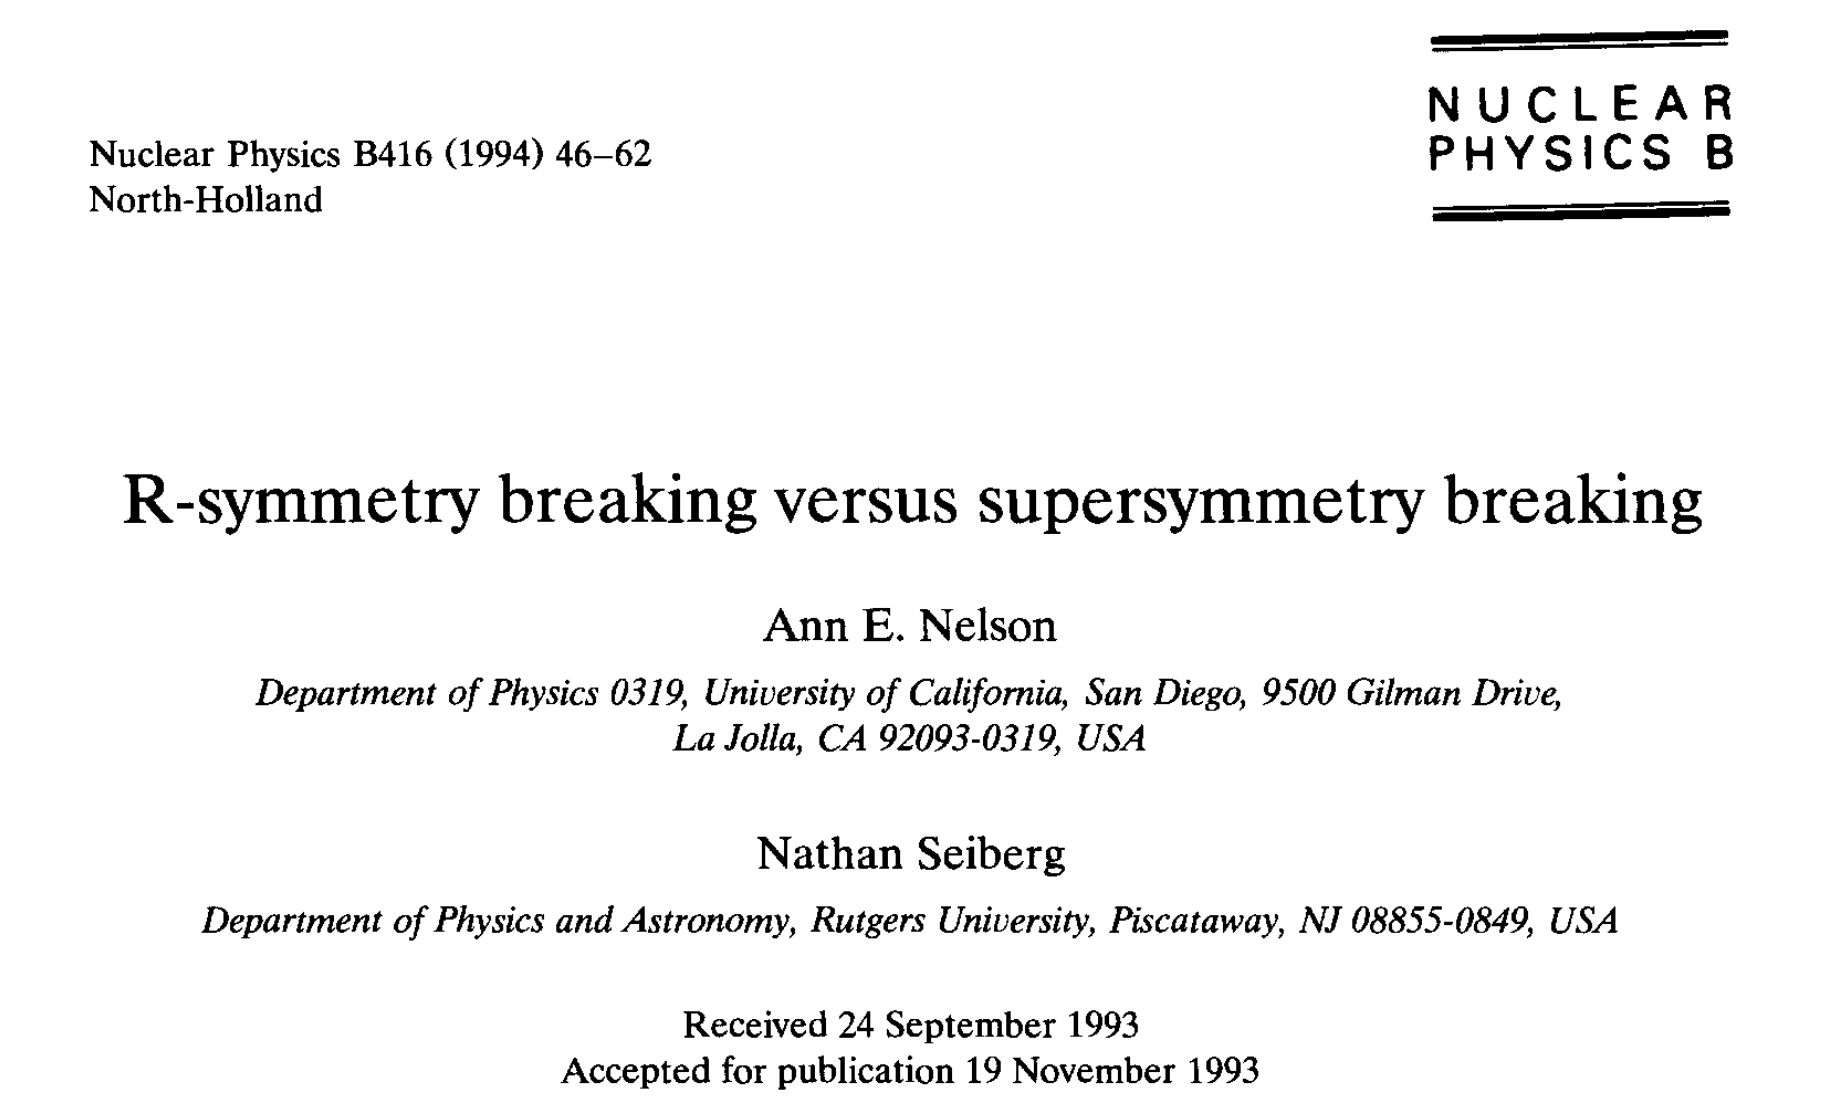
\includegraphics[width=0.6\textwidth]{fig/Nelson1993nf.PNG}
  \end{figure}

  \begin{center}
    (安倍研のActivityで紹介したものです。)
  \end{center}

\end{frame}

\begin{frame}
  \citefone{Shih:2007av}{D. Shih, JHEP 02 (2008) 091}
  \setbeamertemplate{blocks}[rounded][shadow=true]
  \setbeamercolor{block body}{bg=red!10!white, fg=black}
  \begin{block}{}
    \centering
    「\textcolor{DarkMagenta}{R対称性の破れ}」
    $\implies$
    「\textcolor{Goldenrod}{超対称の破れ}」
  \end{block}

  先ほど紹介した論文に関連して、以下の論文を読む\cite{Shih:2007av}。

  \begin{figure}
    \centering
    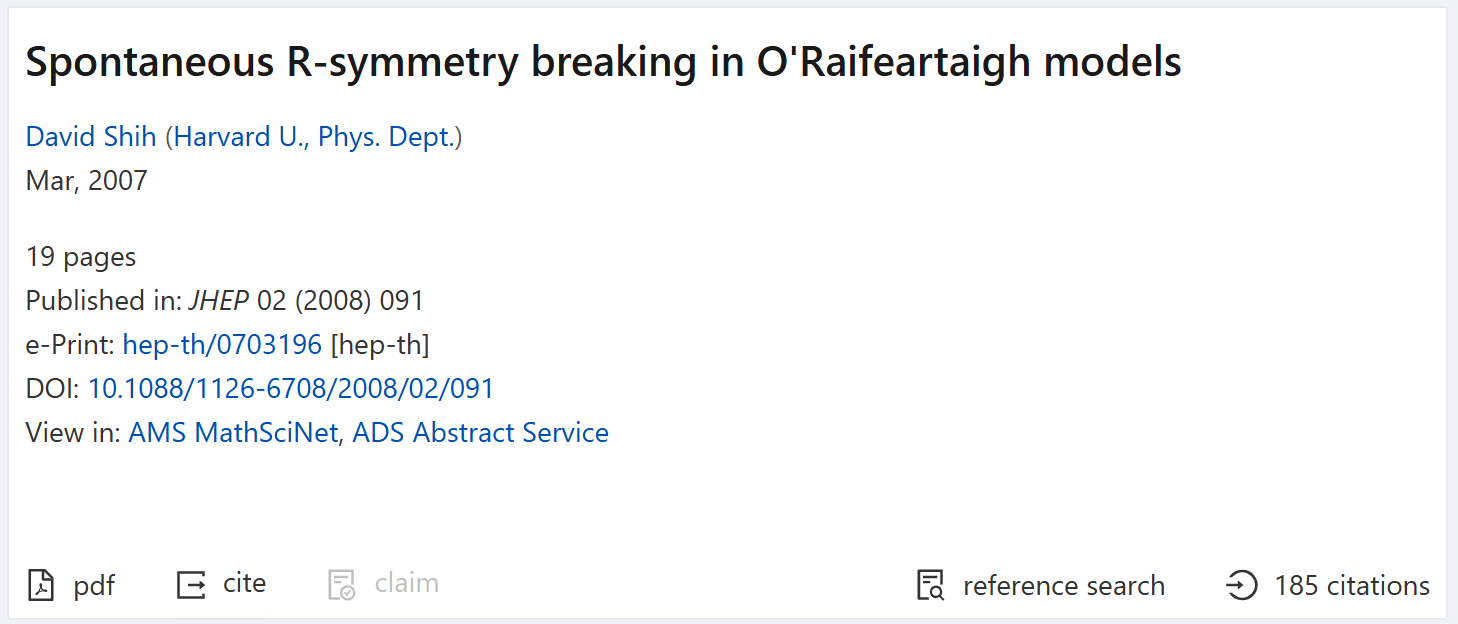
\includegraphics[width=0.6\textwidth]{fig/Shih2007av.PNG}
  \end{figure}

  \uline{論文の概要}

  \begin{itemize}
    \item
          Nelson\ \& Seibergによれば、SUSYを破るためには、(R対称性を理論がもっているなら)それを破らなくてはならない。
    \item
          この論文では、\textcolor{FireBrick}{モデルの摂動ダイナミクス自体}(量子補正)でR対称性を破ることを考える。
    \item
          また、R電荷に条件がつくことが分かる。
  \end{itemize}

\end{frame}

% ----------------------------------------------------------------------------------------------

\section{イントロダクション}

\begin{frame}[plain]
  \huge \secname
\end{frame}


\begin{frame}
  \frametitle{自発的対称性の破れ}

  $n$個の場$\textcolor{DarkGreen}{\Phi_{i}(x)}$が作るポテンシャル$V(\textcolor{DarkGreen}{\Phi_{1},\cdots,\Phi_{n}})$の極小値に興味がある。

  その極小な点(準安定点)を真空$\textcolor{RoyalBlue}{\ev*{\Phi_{i}}}$といい、その真空からの揺らぎ$\textcolor{FireBrick}{\tilde{\Phi}_{i}}$を考える。
  \begin{equation}
    \textcolor{DarkGreen}{\Phi_{i}}
    =
    \textcolor{RoyalBlue}{\ev*{\Phi_{i}}}+\textcolor{FireBrick}{\tilde{\Phi}_{i}}
    \nonumber
  \end{equation}

  この揺らぎに対してのポテンシャル$\tilde{V}$は、元のポテンシャル$V$の対称性を保っているとは限らない。
  \begin{equation}
    \tilde{V}(\textcolor{FireBrick}{\tilde{\Phi}_{i}})
    =
    V(\textcolor{RoyalBlue}{\ev*{\Phi_{i}}}+\textcolor{FireBrick}{\tilde{\Phi}_{i}})
    \nonumber
  \end{equation}
  \begin{center}
    $\longrightarrow$\ 「対称性が自発的に破れている」という。
  \end{center}

  \pause

  もし、場の真空期待値が$0\ (\textrm{i.e.\ } \ev*{\Phi_{i}}=0)$なら、(tree levelでは)対称性は保たれる。
  \begin{equation}
    \tilde{V}(\tilde{\Phi}_{i})
    =
    V(\textcolor{gray}{\ev*{\Phi_{i}}+}\tilde{\Phi}_{i})
    。
    \nonumber
  \end{equation}

\end{frame}

\begin{frame}
  \frametitle{超対称性}

  カイラル多重項$\Phi=\{\phi,\psi,F\}$。この多重項に含まれている粒子の間を
  \begin{equation}
    \textcolor{DarkMagenta}{\xi Q}\phi
    =
    \sqrt{2}\xi \psi
    \ ,\quad
    \textcolor{DarkMagenta}{\xi Q}\psi
    =
    i\sqrt{2}\sigma^{\mu}\bar{\xi}\partial_{\mu}\phi
    +
    \sqrt{2}\xi F
    \ ,\quad
    \textcolor{DarkMagenta}{\xi Q}F
    =
    i\sqrt{2}\bar{\xi}\bar{\sigma}^{\mu}\partial_{\mu}\psi
    \nonumber
  \end{equation}
  のように変換するのが、(無限小)\textcolor{Goldenrod}{超対称変換}。

  この変換で不変な理論のことを\textcolor{Goldenrod}{超対称な理論}と言う。

  \vspace*{15pt}

  また、超対称性を考えるときに、反可換な座標$\theta$を用いた超場形式を用いると、ミンコフスキー時空とグラスマン座標$\theta$を合わせた超空間$(x^{\mu},\theta,\bar{\theta})$が超対称変換の表現空間となっている。
  \begin{gather}
    \Phi
    =
    \phi(x)+i\theta\sigma^{\mu}\bar{\theta}\partial_{\mu}\phi(x)+\frac{1}{4}\theta\theta\overline{\theta\theta}\partial^{2}\phi(x)
    \nonumber
    \\
    \hspace*{1.5cm}
    +\sqrt{2}\theta\psi(x)-\frac{i}{\sqrt{2}}\theta\theta\partial_{\mu}\psi\sigma^{\mu}\bar{\theta}+\theta\theta F(x)
    \nonumber
    \\
    Q_{\alpha}
    =
    \pdv{}{\theta^{\alpha}}
    -
    i\sigma_{\alpha\dot{\alpha}}^{\mu}\partial_{\mu}
    \nonumber
  \end{gather}

\end{frame}

\begin{frame}

  超場によって構成される以下のポテンシャルを考えると超対称な理論が得られる。
  \begin{itemize}
    \item
          \uline{$W$:超ポテンシャル} $\ \rightarrow\ $ 超場の正則な関数で書かれたもの。
    \item
          \uline{$K$:ケーラーポテンシャル} $\ \rightarrow\ $ 実超場によって書かれたもの。
  \end{itemize}

  ラグランジアンは$W, K$に含まれているグラスマン座標を積分して取り除くことで得られる。
  \begin{equation}
    \mathcal{L}
    =
    \int\dd^4\theta\ K(\Phi,\Phi^{\dag})
    +
    \left[
      \int\dd^2 \theta\ W(\Phi)
      +
      \textrm{h.c.}
      \right]
    \nonumber
  \end{equation}

\end{frame}



\begin{frame}
  \frametitle{今回考える理論 (O'Raifeartaigh模型)}

  次の理論を考える。
  \begin{equation}
    \left\{
    \begin{alignedat}{1}
      W
      &=
      fX
      +
      \frac{1}{2}(M_{ij}+XN_{ij})\phi_{i}\phi_{j}
      \\
      K
      &=
      X^{\dag}X
      +
      \phi^{\dag}_{i}\phi_{i}
    \end{alignedat}
    \right.
    \nonumber
  \end{equation}
  ただし、$X,\phi_{i}$はいずれもカイラル超場。

  この理論が次の変換で不変であることを仮定する(\textcolor{DarkRed}{R対称性})
  \begin{equation}
    X\rightarrow e^{2i\alpha}X
    \ ,\quad
    W\rightarrow e^{2i\alpha}W
    \nonumber
  \end{equation}
  (上の仮定から$\phi_{i}\rightarrow e^{iq_{i}\alpha}\phi_{i}$と変換したときの$q_{i}$が決まってくる。が、後で。)

  この理論の真空は
  \begin{equation}
    V_{0}=f^2
    \ ,\quad
    \ev*{\phi_{i}}
    =
    0
    \ ,\quad
    \ev*{X}
    =
    \textrm{\ 任意の定数\ }
    \nonumber
  \end{equation}

  $X$の真空期待値は任意(擬モジュライ)なので、$\ev*{X}=0$とすればR対称性は保たれてしまう。(\uline{c.f.}\ $\ev*{\Phi_{i}}=0$なら$\tilde{V}(\tilde{\Phi}_{i})=V(\textcolor{gray}{\ev*{\Phi_{i}}+}\tilde{\Phi}_{i})$。)

\end{frame}

\begin{frame}
  \frametitle{今回の論文の目的}

  したがって、\uwave{場$X$について}はポテンシャルが\textcolor{red}{立ち上がらない}。
  \begin{equation}
    V(X)
    =
    V_{0}
    +
    \textcolor{gray}{m_{X}^2}|X|^2
    +
    \mathcal{O}(|X|^4)
    \nonumber
  \end{equation}

  \pause

  そこで、今回は
  \setbeamertemplate{blocks}[rounded][shadow=true]
  \setbeamercolor{block body}{bg=red!10!white, fg=black}
  \begin{block}{}
    \centering
    量子補正(Coleman-Weinbergポテンシャル)で$m_{X}^2$を計算\\
    ${\big \Downarrow}$\\
    R対称性を自発的に破る
  \end{block}
  ことを考える。

  \begin{itemize}
    \item
          R対称性が自発的に破れるためには、$m_{X}^2$の符号が負であることが必要\\
          $\ \longrightarrow\ $ $\phi_i$のR電荷$q_{i}$に条件がつく。
    \item
          論文では、$|X|^4$の係数が計算されていなかった。\\
          具体例を見ていったときに、正であることは確認されていたが、一般にそうなっているのか?
  \end{itemize}

\end{frame}

\section{本論}

\begin{frame}[plain]
  \huge \secname
\end{frame}

\begin{frame}
  \frametitle{超対称性の破れ}

  今回考える理論。
  \begin{equation}
    W
    =
    fX
    +
    \frac{1}{2}(M_{ij}+XN_{ij})\phi_{i}\phi_{j}
    \nonumber
  \end{equation}

  $M,N$は複素対称行列。$\det M\neq 0$、$f> 0$を仮定。

  また、$M$を次の形で書く。$M_{i}$はR電荷が$q_{i}$の場の質量行列。
  \begin{equation}
    M
    =
    \begin{pmatrix}
                &           &       &       &       & M_{1} \\
                &           &       &       & M_{2} &       \\
                &           &       & \cdot &       &       \\
                &           & \cdot &       &       &       \\
                & M_{2}^{T} &       &       &       &       \\
      M_{1}^{T} &           &       &       &       &
    \end{pmatrix}
    \nonumber
  \end{equation}

  R対称性を課すと、R電荷に条件がつく。
  \begin{equation}
    M_{ij}\neq 0
    \implies
    R(\phi_{i})+R(\phi_{j})=2
    \ ,\quad
    N_{ij}\neq 0
    \implies
    R(\phi_{i})+R(\phi_{j})=0
    \nonumber
  \end{equation}

\end{frame}

\begin{frame}

  $F$-termのSUSY条件は
  \begin{equation}
    \pdv{W}{\phi_{i}}
    =
    0
    \implies
    (M_{ij}+XN_{ij})\phi_{j}
    =
    0
    \quad
    (j=1,\cdots,n)
    \nonumber
  \end{equation}

  方程式を満たす$\ev*{\phi_{i}}$が存在するかどうか$\ \rightarrow\ \det(M+XN)$を計算\\
  (\uline{c.f.}\ $\det\exp A=\exp\tr A$)
  \begin{align}
    \det (M+XN)
     & =
    \exp\left[ \Tr\ln (1+XM^{-1}N) \right]\det M
    \nonumber
    \\
     & =
    \exp\left[
      -\sum_{k=1}^{\infty}\frac{(-X)^{k}}{k}\Tr(M^{-1}N)^{k}
      \right]
    \det M
    \nonumber
    \\
     &
    =
    \det M\neq 0
    \nonumber
  \end{align}
  最後の等式は\uwave{R電荷の条件}から$\Tr (M^{-1}N)$が$0$となることを用いている。
  \begin{equation}
    \left(
    M_{ij}\neq 0
    \implies
    R(\phi_{i})+R(\phi_{j})=2
    \ ,\quad
    N_{ij}\neq 0
    \implies
    R(\phi_{i})+R(\phi_{j})=0
    \right)
    \nonumber
  \end{equation}

  \begin{center}
    {\Huge $\Downarrow$}\\
    よって、非自明な超対称性を破る真空は存在しない。
  \end{center}

\end{frame}

\begin{frame}
  \frametitle{\texorpdfstring{$m_{X}^2$}{mX^2}の計算}

  Coleman-Weinbergポテンシャルを展開して、$|X|^2$の係数を探る。
  \begin{equation}
    V_{\textrm{eff}}^{(1)}
    =
    \frac{1}{64\pi^2}
    \Tr (-1)^{F}
    \mathcal{M}^{4}\ln\frac{\mathcal{M}^2}{\Lambda^{2}}
    \nonumber
  \end{equation}
  $\Tr (-1)^{F}$は超トレース。$\mathcal{M}$は、スカラーかフェルミオンの質量行列で
  \begin{align}
    \mathcal{M}_{B}^2
     & =
    \begin{pmatrix}
      W^{\dag}_{ik}W^{kj} & W^{\dag}_{ijk}W^{k} \\
      W^{ijk}W_{k}^{\dag} & W^{ik}W_{kj}^{\dag}
    \end{pmatrix}
    =
    (\hat{M}+X\hat{N})^2+f\hat{N}
    \nonumber
    \\
    \mathcal{M}_{F}^2
     & =
    \begin{pmatrix}
      W^{\dag}_{ik}W^{kj} & 0                   \\
      0                   & W^{ik}W_{kj}^{\dag}
    \end{pmatrix}
    =
    (\hat{M}+X\hat{N})^2
    \nonumber
  \end{align}
  ただし、$W_{i}\equiv\partial W/\partial\phi_{i}$。これがスカラーやフェルミオンの質量行列というのは、

\end{frame}


\begin{frame}

  ここで、ポテンシャルの公式を書き換える。
  \begin{equation}    
    \frac{1}{64\pi^2}
    \Tr (-1)^{F}
    \mathcal{M}^{4}\ln\frac{\mathcal{M}^2}{\Lambda^{2}}
    =
    -\frac{1}{32\pi^2}
    \Tr\int^{\Lambda}_{0}\dd v\ 
    v^5\left( \frac{1}{v^2+\mathcal{M}_{B}^2}-\frac{1}{v^2+\mathcal{M}_{F}^2} \right)
    \nonumber
  \end{equation}
  
  ---------------------------------------------------------------------------------

  積分の部分は以下のようになっている。
  \begin{equation}
    \int\dd v\ 
    \frac{v^5}{v^2+\mathcal{M}^2}
    =
    -\frac{1}{2}\mathcal{M}^2 v^2
    +
    \frac{1}{4}v^4
    +
    \frac{1}{2}\mathcal{M}^4\ln(\mathcal{M}^2+v^2)
    \nonumber
  \end{equation}

  あとは$\ln \Lambda^2$で発散する項をみて
  \begin{align}
    \left[  
      \frac{1}{2}\mathcal{M}^4\ln(\mathcal{M}^2+v^2)      
    \right]_{0}^{\Lambda}
    &=
    \frac{1}{2}\mathcal{M}^4\ln\left( 1+\frac{\Lambda^2}{\mathcal{M}^2} \right)
    \nonumber
    \\
    &\sim
    -
    \frac{1}{2}\mathcal{M}^4\ln\frac{\mathcal{M}^2}{\Lambda^2}
    \nonumber
  \end{align}

\end{frame}

\begin{frame}

  

\end{frame}










\section{まとめ}

\begin{frame}[plain]
  \huge \secname
\end{frame}


\begin{frame}
  \frametitle{まとめ}










\end{frame}


% --------------------------

\newcounter{Appendix}
\setcounter{Appendix}{\value{framenumber}}
\setcounter{section}{0}
\renewcommand{\thesubsection}{\Alph{subsection}}
\makeatletter
\renewcommand{\theequation}{\thesubsection.\arabic{equation}}
\@addtoreset{equation}{section}

\renewcommand{\thefigure}{\thesubsection.\arabic{figure}}
\@addtoreset{figure}{section}

\renewcommand{\thetable}{\thesubsection.\arabic{table}}
\@addtoreset{table}{section}
\makeatother

\section{付録}

\begin{frame}[plain]
  \frametitle{\ }
  \huge \secname
\end{frame}

\subsection{目次}

\begin{frame}[plain,allowframebreaks]{\subsecname}
  \tableofcontents
\end{frame}



% --------------------------

\section{参考文献}
\begin{frame}[plain,allowframebreaks]{\secname}

  \scriptsize
  \beamertemplatetextbibitems
  \bibliographystyle{ytphys}
  \bibliography{ref}

\end{frame}

\setcounter{framenumber}{\value{Appendix}}
\end{document}
